\documentclass[11pt]{article}

% ---------------------------------------------------------------------------
% The Value of the Marginal Solver
% Reflowed to the CVA CFP 2026 / Ledger journal house style (see README.md):
% Times New Roman 11.5/13.5, 3.1 cm side margins, 13 pt bold numbered section
% headings, inline italic em-dash subheadings, numbered superscript endnote
% citations in a "Notes and References" section.
% Single-author paper; first-person singular voice (academic-writing-style.md).
% ---------------------------------------------------------------------------

\usepackage[utf8]{inputenc}
\usepackage[T1]{fontenc}
\usepackage[a4paper,left=3.1cm,right=3.1cm,top=2.4cm,bottom=1.0cm,
            headheight=14pt,headsep=0.7cm,footskip=0.6cm]{geometry}
\usepackage{amsmath,amsthm}
\usepackage{newtxtext,newtxmath}   % Times New Roman-like text and math
\usepackage{booktabs}
\usepackage{graphicx}
\usepackage{microtype}
\usepackage[super,numbers,sort&compress]{natbib}
\usepackage[explicit]{titlesec}
\usepackage{fancyhdr}
\usepackage[hidelinks]{hyperref}

% --- Ledger body font size: 11.5 pt on 13.5 pt leading --------------------
\makeatletter
\renewcommand\normalsize{%
  \@setfontsize\normalsize{11.5pt}{13.5pt}%
  \abovedisplayskip 10\p@ \@plus3\p@ \@minus6\p@
  \belowdisplayskip \abovedisplayskip
  \abovedisplayshortskip \z@ \@plus3\p@
  \belowdisplayshortskip 6.5\p@ \@plus3.5\p@ \@minus3\p@}
\makeatother
\normalsize

% --- Section headings: 13 pt Times bold, numbered with a period -----------
\titleformat{\section}
  {\normalfont\bfseries\fontsize{13}{15}\selectfont}{\thesection.}{0.6em}{#1}
\titlespacing*{\section}{0pt}{2.2ex plus 1ex minus .2ex}{1.0ex}

% --- Numbered subheadings: inline, italic, followed by an em dash ----------
\titleformat{\subsection}[runin]
  {\normalfont\itshape}{\upshape\thesubsection}{0.5em}{#1}[\textup{---}]
\titlespacing*{\subsection}{0pt}{1.3ex plus .3ex}{0.15em}

% --- Run-in topic heads: inline, italic, followed by an em dash ------------
\titleformat{\paragraph}[runin]
  {\normalfont\itshape}{}{0pt}{#1}[\textup{---}]
\titlespacing*{\paragraph}{0pt}{1.1ex plus .2ex}{0.15em}

% --- Running head and page number (Ledger) --------------------------------
\pagestyle{fancy}
\fancyhf{}
\fancyhead[C]{\fontsize{10}{12}\selectfont CVA Academic Research Journal 2026}
\fancyfoot[L]{\fontsize{10}{12}\selectfont\thepage}
\renewcommand{\headrulewidth}{0pt}
\fancypagestyle{plain}{\fancyhf{}%
  \fancyhead[C]{\fontsize{10}{12}\selectfont CVA Academic Research Journal 2026}%
  \fancyfoot[L]{\fontsize{10}{12}\selectfont\thepage}%
  \renewcommand{\headrulewidth}{0pt}}

% References appear as a numbered "Notes and References" section (Ledger).
\renewcommand{\refname}{Notes and References}

\theoremstyle{plain}
\newtheorem{proposition}{Proposition}
\newtheorem{corollary}{Corollary}
\theoremstyle{definition}
\newtheorem{definition}{Definition}
\theoremstyle{remark}
\newtheorem{remark}{Remark}

\newcommand{\E}{\mathbb{E}}
\newcommand{\Prb}{\mathbb{P}}
\newcommand\blfootnote[1]{\begingroup\renewcommand\thefootnote{}%
  \footnotetext{#1}\addtocounter{footnote}{-1}\endgroup}

\begin{document}

% --- Title block (Ledger: 24 pt centered title, 13 pt author) --------------
\thispagestyle{plain}
\begin{center}
{\fontsize{24}{28}\selectfont The Value of the Marginal Solver:\\[2pt]
Competition and Best Execution\\ in Intent-Based Markets\par}
\vspace{1.4em}
{\fontsize{13}{16}\selectfont Nils Bundi\textsuperscript{*,\,1}\par}
\end{center}
\blfootnote{\fontsize{8}{9}\selectfont\textsuperscript{1}N.\ Bundi (\texttt{bund@zhaw.ch}) is a researcher at the Zurich University of Applied Sciences (ZHAW), Switzerland. \textsuperscript{*}Corresponding author.}
\vspace{0.4em}

% --- Abstract (Ledger: 10 pt, 1.2 cm side indents, bold run-in "Abstract.")
{\fontsize{10}{13}\selectfont
\setlength{\leftskip}{1.2cm}\setlength{\rightskip}{1.2cm}
\noindent\textbf{Abstract.}\quad What is one more competitor for a customer order worth? The question is as old as market microstructure and has never met a computed counterfactual: the losing bids were never public in the markets that debated it. I assemble the complete bid record of the first production market, to my knowledge, to publish its losing bids: 565{,}259 CoW Protocol batch auctions, twelve months, 692{,}964 orders, 47 solvers. With bids held fixed, thinning an order's field becomes computable; the schedule is Stigler's value-of-search curve drawn from observed quotations: a single retained bidder costs the median order 14 basis points, a second restores 8, a fifth less than 1 (medians). The data then reject both poles of existing entry theory. Leadership is persistently concentrated in asset niches, against symmetric-entry models; yet when leading solvers exited, their niches were reoccupied within a month at no relative cost, against firm-attached asymmetry; and a reward reform moved participation, never bids. I propose the reconciliation: execution capacity attaches to positions that symmetric firms occupy under entry costs, so positions are contestable while aggregate depth adjusts slowly. Competition matters; competitors are replaceable; the depth of the field is the statistic that prices it.
\par}

\vspace{0.7em}
{\fontsize{10}{13}\selectfont
\begin{center}KEY WORDS\end{center}
\vspace{-0.4em}
\begin{center}
1.~Solver competition.\quad 2.~Order flow auctions.\quad 3.~Best execution.\quad 4.~Batch auctions.\quad 5.~Market microstructure.
\end{center}
}
\vspace{0.5em}

% ===========================================================================
\section{Introduction}
% ===========================================================================

This paper asks \emph{what one more competitor for a customer order is worth}. The question is among the oldest in market microstructure. Demsetz founded the field on the observation that transacting costs are prices set by suppliers of immediacy competing for order flow~\citep{demsetz1968cost}. The theory of dealership predicts that competition among those suppliers narrows what customers pay~\citep{ho1983dynamics}, while mechanism-design theory predicts that rents survive any finite amount of it~\citep{biais2000competing}. Auction theory elevated the question to a design principle: under standard conditions, an auction with one additional bidder outperforms the optimal mechanism without that bidder~\citep{bulow1996auctions}. Yet the empirical record is indirect and famously contradictory. Execution costs decline in dealer counts in some markets, and dealer responses to electronic bond inquiries lower costs as they multiply~\citep{hendershott2015click}, while NASDAQ sustained collusive spreads with thirty quoting dealers per stock~\citep{christie1994nasdaq}. The object the question turns on, the offers an order \emph{could} have had but did not take, has been visible at best in fragments, confidential response sets on single platforms, winning bids in auction records, so fifty years of answers have been inferences from spreads, counts, and structural models, not public measurements of the counterfactual.

This paper measures the counterfactual. A new class of market infrastructure makes it possible. In intent-based settlement, a user signs a declarative order and professional \emph{solvers} bid to execute it in discrete batch auctions, a design descended from the frequent batch auction proposed as the remedy for speed races~\citep{budish2015hft} and deployed on-chain to shield users from the extractable value of transparent execution~\citep{daian2020flashboys}. Every few seconds the protocol collects signed orders into a batch, broadcasts it to bonded solver firms, and settles the winning proposals on-chain; users trade against an auction, not against a book, and no broker stands in between. That last fact raises the stakes beyond one venue: where a broker would owe the best-execution duty of MiFID~II, FinSA, or FINRA Rule~5310~\citep{mifid2,finsa,finra5310}, here competition among solvers is the duty's only functional substitute, so what that competition is worth is not merely a market-design question but the operative question of investor protection. The largest such venue, CoW Protocol, settled about \$87~billion in 2025~\citep{cowdao_review2025}, and it does something that, to my knowledge, no production financial market has done before: for every auction it publishes every submitted bid, losers included, with bidder identity and proposed execution~\citep{cow_api}. From this record I assemble a census of 565{,}259 auctions on Ethereum mainnet over twelve months, covering 692{,}964 settled orders and every offer that 47 distinct solvers made for them.

Two features make this record unusually well suited to the question. First, it is complete and public, where the treasury-auction literature's bid data reach the econometrician confidentially and strategically shaded~\citep{hortacsu2010mechanism,kastl2011discrete}. Second, the venue's reward rule pays winners by their margin over the runner-up, a design that pushes bids toward deliverable executions, so on the recorded bids the counterfactual of thinning an order's field can be computed directly, a finite-population calculation over the offers actually submitted. Whether the fixed-bid counterfactual approximates the equilibrium one is a real question, and the paper confronts it with realized outcomes.

I give four answers. First, the value of competition: a single retained bidder, bids held fixed, costs the median order 14 basis points, a second restores 8, a fifth less than 1, the front-loaded Stigler value-of-search schedule drawn from submitted quotations and monotone in liquidity, from 96 basis points in the thinnest asset quintile to 14 in the deepest. The next three adjudicate a theory. Second, leadership is persistent and niche-specific: of 47 solvers, 21 lead at least one asset and the busiest leads only a third, so bidders are not the exchangeable draws of symmetric-entry models~\citep{levin1994entry}. Third, that heterogeneity does not attach to the firm either: when three leading solvers exited in December 2025, the niches they had dominated were reoccupied within a month and their execution did not deteriorate relative to unexposed assets, against the firm-attached asymmetry~\citep{maskin2000asymmetric} that predicts a strong bidder's exit is costly. Fourth, a reward reform in the same month moved participation but never bids. I reconcile all four with a minimal extension of costly-entry auction theory: execution capacity attaches to \emph{positions}, asset niches that ex-ante symmetric firms occupy under entry costs, so competition for the position disciplines outcomes in it while firms remain replaceable occupants. The fixed-bid measure is therefore an upper bound on realized dependence, positions are contestable, and what binds is aggregate depth: competition matters, competitors are replaceable.

\emph{Contributions.} The paper contributes the measure, a finite-population value of competition computed directly from the first complete public bid record I am aware of; the two experiments that discipline it, showing exposure washes out through substitution while rewards act on participation, not bids; and an extension of costly-entry auction theory that the data force. Persistent niche leadership rejects symmetric entry, exit-neutrality rejects firm-attached asymmetry, and the minimal reconciliation, capacity that attaches to positions which symmetric firms occupy under entry costs, replicates the market's cross-section and dynamics and renders positions contestable while aggregate depth adjusts slowly. The monitoring implication follows: in broker-free markets the depth of the field is the summary statistic that moves with execution quality, auditable from public data.

\emph{Organization.} Section~2 locates the paper and names the gaps it closes; Section~3 describes the auction, the census, and the bid panel; Section~4 sets out the model whose propositions organize the empirics; Section~5 reports the results in the order of the four answers; Sections~6 to~8 discuss implications, limitations, and conclusions.

% ===========================================================================
\section{Related Literature and Contribution}
% ===========================================================================

\paragraph{The value of competition for order flow} The question is a classic with an unresolved empirical record. \citet{demsetz1968cost} cast the bid--ask spread as the price of immediacy, disciplined by competition among its suppliers; \citet{ho1983dynamics} model competing dealers and predict that customer costs fall as their number rises; \citet{biais2000competing} show that even under competition among many liquidity suppliers, informational rents survive in equilibrium. The evidence has been unable to separate these forces cleanly. \citet{christie1994nasdaq} showed that thirty quoting dealers per NASDAQ stock sustained spreads consistent with implicit collusion, so the count of competitors, the variable every study must use, does not by itself measure competition. The closest antecedents are in the request-for-quote literature: \citet{hendershott2015click} observe competing dealer responses to electronic bond auctions in proprietary platform data and show that prices improve with the number of responses, and \citet{riggs2020swap} observe the full trade-formation record on swap execution facilities, losing quotes included, down to the distance between the best and second-best response. That work establishes the gradient and even the margin; the counterfactual remained out of reach, since the data are proprietary to one platform's solicited flow and, as \citet{hendershott2015click} themselves model, both the number of dealers contacted and the number responding are endogenous choices, so removing a responder is not a computable experiment there. What has been missing, to my knowledge, in every market where the question has been debated is a public, venue-wide record of the losing side, complete enough that thinning the field becomes a computable counterfactual. This paper's market publishes exactly that.

\paragraph{Auctions, search, and bid data} Auction theory supplies the framework: truthful bidding under runner-up pricing is Vickrey's result~\citep{vickrey1961counterspeculation}, and \citet{bulow1996auctions} prove, for symmetric independent private values, that an English auction with one extra bidder dominates the optimal mechanism without him, the formal core of the folk principle that attracting bidders beats refining rules. The same object anchors the economics of information: the expected best price from $m$ quotations is Stigler's value-of-search curve~\citep{stigler1961information}, with the equilibrium price dispersion that sustains it supplied by \citet{burdett1983dispersion}. Price-dispersion studies then measured pieces of the curve from collected quotations: \citet{pratt1979price} its endpoints, the gain from full search over a single draw, and \citet{baye2004price} the winner--runner-up gap against the number of listed sellers. This paper draws the full curve, at every $m$, from each order's own observed field. Empirical auction economics has analyzed full bid data before, notably in treasury markets~\citep{hortacsu2010mechanism,kastl2011discrete}, but the two settings differ from the request-for-quote evidence above and from each other: treasury auctions are divisible-good sales by a single issuer whose full bid schedules reach the econometrician under confidentiality, and their discriminatory or uniform pricing makes bids strategically shaded, so counterfactuals require structural estimation. Here the record is public and the reward rule pushes bids toward face value. The venue's mechanism descends from a second lineage, the frequent batch auction proposed as a remedy for the continuous market's speed race~\citep{budish2015hft,aquilina2022quantifying}, here running at scale on a blockchain because batching also internalizes the extractable-value problem of transparent on-chain execution~\citep{daian2020flashboys}.

\paragraph{Intent venues: measurement and market structure} A young literature measures solver-based venues from the user's side: \citet{bachu2024quantifying} benchmark executed orders against a routed counterfactual and find price improvement of a few basis points, \citet{yuminaga2025welfare} compare venues across liquidity tiers, and \citet{watts2025failure} study execution guarantees in permissionless order-flow auctions. All condition on winning executions. On the supply side, \citet{chitra2024intent} model solver entry costs and predict equilibrium oligopoly, and \citet{zhang2026incentives} studies the CIP-74 reward reform through concentration indices built from winning bids, finding shifting shares with no detectable change in execution quality within roughly seven basis points. A parallel blockchain literature studies block-builder auctions, whose relay archives also expose bids: \citet{yang2024builder} compute a winner-versus-runner-up competitiveness index on MEV-Boost data, \citet{pahari2025exclusive} exploit non-winning block submissions, and theory examines builder centralization~\citep{bahrani2024pbs,gupta2023centralizing}; block building, however, auctions one homogeneous slot rather than executions for individual customer orders, and none of this work computes bid-thinning counterfactuals. On the intent venues themselves, bid-level analysis was never assembled. The bid panel measures what structure only proxies, the price distance between the winner and the field, and speaks to the mechanism behind Zhang's no-change finding: a reform that moved participation but not conditional margins. A final strand asks who provides liquidity at all, with symmetric costly entry~\citep{mcafee1987entry,levin1994entry}, firm-attached asymmetry~\citep{maskin2000asymmetric}, and role-formation models~\citep{atkeson2015entry,farboodi2023emergence,sambalaibat2025clienteles} as its poles; Section~\ref{sec:model-positions} locates the paper's extension in that chain and the exit and reform evidence adjudicates among them.

\paragraph{Mechanism design and the missing empirics} \citet{canidio2024fair} design the fair combinatorial auction that CoW adopted in 2025~\citep{cowdao_fairauction}: solvers bid on single orders and on batches, and batched bids are filtered against a reference outcome constructed from the bids themselves. The design trades batching efficiencies against per-order optimality, and my data prices both sides of that trade-off in production. On the regulatory side, recent legal scholarship argues that verifiable on-chain execution could discharge best-execution-type duties by design~\citep{le2026fairness}; what that argument lacks is measurement, and the present paper supplies the measured object, competition, on which any such discharge would rest.

Two gaps emerge from these four strands. First, no study I am aware of, in any market, has measured the value of a competitor for order flow against a computed rather than estimated counterfactual, because no market published a complete bid record; the RFQ evidence comes closest and stops at confidential response counts. Second, the mechanism-design and regulatory strands both presuppose a quantity, the execution quality that competition delivers, that the measurement strands have not supplied. The present paper closes both gaps with the same object, the complete bid panel of a production auction market, and then tests the fixed-bid measure against realized outcomes.

% ===========================================================================
\section{The Auction, the Census, and the Bid Panel}
% ===========================================================================

\subsection{The venue}\label{sec:venue}
CoW Protocol clears trades in discrete auctions. The protocol collects signed intents into a batch, broadcasts the batch to a permissioned but open set of bonded solvers, receives competing settlement proposals, and selects winners under the fair combinatorial auction adopted in 2025: solvers submit bids on individual orders and on batches, the best individual-order bids define a reference outcome per directed token pair, and batched bids that would leave any trade worse than its reference are filtered out~\citep{cowdao_rules,cowdao_fairauction}. Winning solvers are rewarded by a second-price-flavoured rule keyed to the margin of their score over the runner-up's, subject to caps~\citep{cowdao_rewards}. On 8~December 2025, inside my sample window, governance proposal CIP-74 re-tied the reward cap to protocol revenue and introduced a volume-based fee, repricing participation without changing the allocation rule~\citep{zhang2026incentives}. Critically for this paper, the protocol publishes the entire solver-competition record for every auction, all submitted solutions, winning and losing, with solver identities, proposed per-order executions, and a native price vector valuing every token in ETH~\citep{cow_api}. By contrast, the per-order Dutch auctions of UniswapX and 1inch Fusion~\citep{adams2023uniswapx} disclose no losing quotes, which is why this measurement is possible only here.

\subsection{Census}\label{sec:census}
I collect every settlement auction on Ethereum mainnet from 12~August 2025 to 15~August 2026: 565{,}259 auctions containing 692{,}964 settled orders quoted against USDC. Restricting to USDC-quoted orders fixes a common numeraire. Orders are stratified by a liquidity metric computed from the census itself: each counter-asset's total ETH volume over the sample, on a log scale, cut into asset quintiles L1 (thinnest) through L5 (deepest). Because volume concentrates in few assets, the deepest quintile carries most orders; per-quintile composition appears in Table~\ref{tab:field}. An auxiliary dataset completes the record: for 509{,}309 executed orders I hold a counterfactual quote from the Uniswap smart-order router, pinned to the order's settlement block, together with per-block base fees to net out the direct-swap gas a settled user avoids. Realized price improvement against this routed benchmark is the realized-quality outcome of the experiments in Section~\ref{sec:results}. Block heights are approximated to calendar time by a linear model anchored at the census's first and last block timestamps, a fair approximation given Ethereum's fixed twelve-second slot schedule.

\subsection{The bid panel}\label{sec:panel}
For each order $i$ in each auction I extract, from every submitted solution, the execution each solver proposed for that order, and keep each solver's best proposal. The offer is summarized by the execution ratio $r = \text{buy}/\text{sell}$, output per unit of input, which is monotone in user welfare and valid for buy and sell orders alike. This yields, per order, the number of distinct competing solvers $n_i$, the ranked offers $r_i^{(1)} \ge r_i^{(2)} \ge \dots \ge r_i^{(n_i)}$, the winning execution, and each offer's solver identity. Two sanity filters guard against non-economic records: offer gaps are winsorized at 2{,}000 basis points, binding on 0.09 percent of orders, and notionals whose native-price valuation exceeds $10^5$~ETH are treated as missing.

\begin{definition}[Runner-up margin]\label{def:gap}
For an order with $n_i \ge 2$ competing solvers, the runner-up margin is
\begin{equation}\label{eq:gap}
\Delta_i \;:=\; 10^4 \cdot \frac{r_i^{(1)} - r_i^{(2)}}{r_i^{(2)}} \quad \text{(bps)},
\end{equation}
the loss the order would suffer, holding bids fixed, if the solver making its best offer did not participate.
\end{definition}

Figure~\ref{fig:anatomy} shows the object for one representative auction: twelve solvers competed for a one-ETH WETH/USDC order, the field's bids cluster within a few basis points of the best losing bid, and the runner-up margin is about one basis point, competition at work in its normal, healthy state. Table~\ref{tab:field} in Section~\ref{sec:results} reports the panel's participation structure.

\begin{figure}[t]
\centering
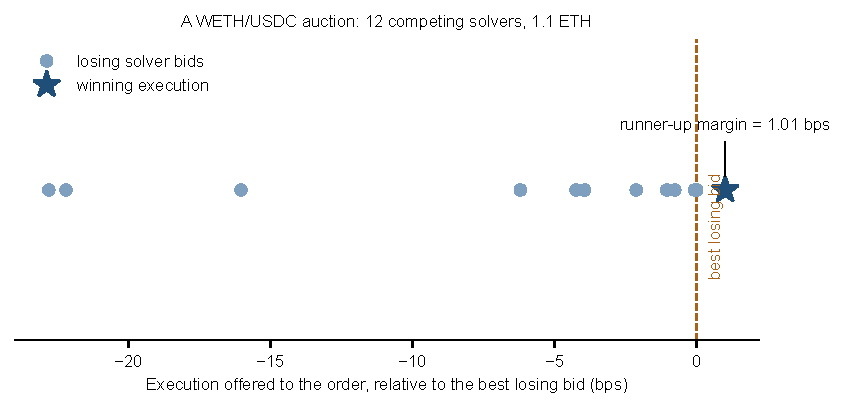
\includegraphics[width=\linewidth]{figures/fig_anatomy.pdf}
\caption{Anatomy of one auction from the census: the bids of twelve competing solvers for a single 1.07~ETH WETH/USDC order, expressed relative to the best losing bid. The winning execution (star) exceeds the best losing bid by a runner-up margin of 1.0 basis points; the remaining field sits within a few basis points, with one distant outlier. Every element of the figure is on the public record.}
\label{fig:anatomy}
\end{figure}

% ===========================================================================
\section{A Model of Solver Competition}
% ===========================================================================

\subsection{Setup and truthful bidding}\label{sec:model-setup}
The model is a deliberate per-order idealization of a batch mechanism. An order $i$ arrives with characteristics (pair, size, liquidity). Each of $n$ participating solvers $j$ has an execution capacity $R_{ij}$, the best ratio it can deliver given its routing technology, inventory, and private liquidity, drawn independently from a distribution $F_i$ whose dispersion $\sigma_i$ reflects how unevenly execution technology applies to the order: for deep assets all solvers find nearly the same route and $\sigma_i$ is small; for thin assets routes differ and $\sigma_i$ is large. In the idealized mechanism, solvers submit bids $b_{ij}$, the order goes to the maximum, and the winner earns a reward increasing in its margin over the runner-up. This is a second-price auction run in scores, and Vickrey's dominant-strategy theorem applies directly~\citep{vickrey1961counterspeculation}: because the winner's payoff turns on the runner-up's bid rather than its own, shading below capacity only forfeits auctions the solver could profitably have won, and overbidding risks winning at an undeliverable execution, so bidding one's capacity, $b_{ij} = R_{ij}$, is dominant. The protocol's own documentation makes the same argument for the production rules~\citep{cowdao_rewards}, and the structure has a dealership ancestor: in the competing-dealer model of \citet{ho1983dynamics} it is likewise the second-best dealer who sets the market spread, so the runner-up margin of Definition~\ref{def:gap} is the auction-market form of an object dealer theory has long placed at the center. The production mechanism departs from this in ways that matter. Selection is batch-level over collections of fair solutions, not per-order; rewards are capped, and the protocol's own documentation notes that the cap introduces first-price incentives and that truthful reporting need not be optimal in uncompetitive auctions~\citep{cowdao_rewards,cowdao_rules}. I therefore treat bids-as-capacities as a \emph{maintained idealization}, not an established fact: it motivates reading the recorded bids as deliverable executions, the empirical objects below are well-defined without it, and Section~\ref{sec:exitstudy} tests its central implication against realized outcomes.

\subsection{The value of the marginal solver}\label{sec:model-value}
Let $V_i(m) = \E\!\left[\max(R_{i1},\dots,R_{im})\right]$ be the expected execution an order receives from $m$ competing solvers, and let $\delta_i(m) = V_i(m) - V_i(m-1)$ be the value of the $m$-th solver.

\begin{proposition}[Diminishing marginal value]\label{prop:diminishing}
$V_i(m)$ is increasing in $m$ and $\delta_i(m)$ is decreasing in $m$: competition's value is front-loaded.
\end{proposition}

\begin{proof}
Write $M_{m-1} = \max(R_{i1},\dots,R_{i,m-1})$. Then $V_i(m) - V_i(m-1) = \E\big[(R_{im} - M_{m-1})^+\big]$, which is positive, and decreasing in $m$ because $M_{m-1}$ is stochastically increasing in $m$ while $R_{im}$ is an independent draw from the same $F_i$.
\end{proof}

\begin{proposition}[Dispersion scaling]\label{prop:dispersion}
If $F_i$ belongs to a location--scale family, $R_{ij} = \mu_i + \sigma_i Z_j$ with $Z_j \sim G$ i.i.d., then $\delta_i(m) = \sigma_i\, d_G(m)$ for a family constant $d_G(m)$: the value of every marginal solver scales with the dispersion of execution capacities.
\end{proposition}

\begin{proof}
$V_i(m) = \mu_i + \sigma_i \E[\max(Z_1,\dots,Z_m)]$; difference in $m$.
\end{proof}

Proposition~\ref{prop:dispersion} is the liquidity prediction: the marginal solver curve should sit higher, at every $m$, where execution capacities disperse more, and lower for larger orders within liquid pairs, which leave less room for technological disagreement per unit of notional. Both propositions are textbook properties of expected maxima~\citep{david2003order}, stated here to fix notation and predictions, not claimed as theory. $V_i(m)$ is, formally, the expected best quotation from $m$ draws, the object on which \citet{stigler1961information} founded the economics of information and whose equilibrium dispersion \citet{burdett1983dispersion} supplied; what that literature lacked is observed quotations to draw the curve from; Section~\ref{sec:curve} draws it.

\subsection{Entry, rewards, and the participation channel}\label{sec:model-entry}
Participation is endogenous. Bidding on an order costs $c$ (infrastructure, computation, inventory reservation), and a solver's expected rent from participating is its probability of winning times the expected reward margin. With free entry the marginal solver's rent equals $c$, pinning down equilibrium participation $n^\ast_i$, the costly-entry formulation of \citet{mcafee1987entry} and \citet{levin1994entry}, in whose zero-profit equilibrium seller policy already reaches outcomes through the participation margin; the entry-cost oligopoly of \citet{chitra2024intent} is the same economics on-chain. Packaging these standard ingredients for the reward-setting problem at hand delivers the model's testable prediction.

\begin{proposition}[Participation channel]\label{prop:neutrality}
Under truthful bidding the reward level does not enter bids, so a change in rewards moves realized execution quality only through equilibrium participation: to first order, quality moves by $\delta_i(n^\ast_i)\,\Delta n^\ast_i$, the marginal solver curve of Proposition~\ref{prop:diminishing} evaluated at the participation change the reform induces.
\end{proposition}

\begin{proof}
Immediate from combining \citet{vickrey1961counterspeculation} with free entry: the truthful bid $b_{ij} = R_{ij}$ does not depend on the reward level, which enters payoffs only as a scaling of the winner's transfer and therefore appears only in the free-entry condition, where a higher expected reward supports a higher $n^\ast_i$ at given cost $c$. A first-order expansion of $V_i(n^\ast_i)$ gives the transmission.
\end{proof}

\begin{remark}[Conditional invariance]\label{rem:invariance}
In the idealized model the proposition has a sharper corollary: the bid distribution, hence the runner-up margin conditional on $n$, is invariant to the reward level. I state the corollary for completeness but do not treat it as testable in field data, because $n$ is an equilibrium object and order composition co-moves with membership, a failure the discussion summarizes; Section~\ref{sec:time} instead tests the proposition through a cross-sectional exposure design that the mechanism itself supplies, since the production reward is capped and, per the protocol's own documentation, truthfulness weakens exactly where the cap binds~\citep{cowdao_rewards}.
\end{remark}

Proposition~\ref{prop:neutrality} is what the model asserts at the level where identification exists: it predicts \emph{where} a reward reform acts (membership and participation) and \emph{how much} quality can move (the curve times the induced participation change). The empirical logic has a named ancestry: \citet{li2009entry} decompose auction policy into entry and competition effects, and \citet{athey2011open} split format effects into participation and bidding margins; in a second-score venue the competition effect on bids is zero under truthfulness, isolating the entry effect. A second comparative static covers exits: in the idealized model, removing draws from the maximum lowers realized execution, symmetrically recovering on entry, and Section~\ref{sec:exitstudy} tests the fixed-bid version of that prediction against realized outcomes. In the spirit of \citet{bulow1996auctions}, the model says a venue gains more from one additional serious solver than from fine-tuning its allocation rule, and Section~\ref{sec:results} reports the field magnitudes relevant to that comparison.

\subsection{Positions, not firms}\label{sec:model-positions}
The benchmark of Sections~4.1--4.3 inherits an assumption the auction literature has already rejected once, and the data of Section~\ref{sec:results} reject twice. Under symmetric entry~\citep{mcafee1987entry,levin1994entry}, bidders are exchangeable and no firm should lead persistently anywhere. The standard repair attaches heterogeneity to the firm~\citep{maskin2000asymmetric}, and its empirical basis is broad: permanent bidder classes in timber auctions~\citep{athey2011open,roberts2013auctions}, incumbency advantages in procurement~\citep{desilva2003entrant}, capacity-state asymmetries~\citep{jofre2003dynamic}. In quote-driven markets the firm-attached view carries a sharp prediction, that losing a particular provider is costly, and the evidence has supported it: dealer exits permanently widen spreads~\citep{wahal1997entry}, removing designated market makers degrades liquidity where removing voluntary providers does not~\citep{clarkjoseph2017designated,venkataraman2007value}, a single market maker can carry a venue~\citep{menkveld2013high}, and providers withdraw together under stress~\citep{anand2016market}. Section~\ref{sec:results} documents both deviations at once in one market: leadership is persistent and niche-specific, against exchangeability, yet the exit of leading firms leaves their niches unharmed, against firm attachment.

I reconcile the two with a minimal reassignment of where heterogeneity lives. Execution technology is instrument-specific in most markets, the integrations, inventory, and information that executing a particular instrument demands, so let each niche $i$ carry its own capacity distribution $F_i$ as a property of the niche, and let ex-ante symmetric firms pay an occupancy cost $\kappa_i$ to hold a position in it, entry into positions as in \citet{salop1979monopolistic}, value attaching to the slot as in position auctions~\citep{edelman2007internet}. Occupants of niche $i$ draw capacities from $F_i$ order by order and compete in the second-score auction of Section~\ref{sec:model-setup}; free occupancy entry pins the number of occupants $n^\ast_i$ niche by niche, exactly as in Section~\ref{sec:model-entry}.

\begin{proposition}[Occupant invariance]\label{prop:occupancy}
In equilibrium the distribution of execution outcomes in niche $i$ depends only on $(F_i, n^\ast_i)$, not on which firms occupy its positions. The exit of an occupant is followed by reoccupation whenever niche rents cover $\kappa_i$, restoring the outcome distribution, and occupancy confers no rent beyond the entry cost.
\end{proposition}

\begin{proof}
Occupants are symmetric within a niche because capacities are draws from the niche's $F_i$; Vickrey pricing ties outcomes to order statistics of those draws alone; and the free-entry condition re-equilibrates $n^\ast_i$ after any exit. The no-rent statement is the zero-profit condition; its spatial ancestor is \citet{judd1985preemption}, where occupancy protects nothing when exit and entry are cheap.
\end{proof}

\begin{remark}[Two speeds]\label{rem:twospeeds}
Reoccupation moves existing capacity across niches at the occupancy margin and is fast; the aggregate stock of capacity, the $\kappa$-funded infrastructure of firms, adjusts at the firm-formation margin and is slow. The model thus separates two objects that the symmetric and firm-attached poles each collapse into one: niche outcomes are \emph{contestable}, disciplined by competition for the position in the sense of \citet{chadwick1859field}, \citet{demsetz1968utilities}, \citet{williamson1976franchise}, and \citet{baumol1982contestable}, while aggregate depth is a slow state variable, the resilience margin that \citet{atkeson2015entry} parameterize. The nearest models deriving persistent heterogeneity from symmetric primitives are \citet{farboodi2023emergence} and \citet{sambalaibat2025clienteles}, where the role is acquired by the firm through investment or clientele sorting; here the role is the position itself and the firm is its transient occupant, with \citet{hugonnier2020frictional} the firm-attached pole in over-the-counter theory. Section~\ref{sec:exitstudy} tests the proposition's signature, exit-neutrality with reoccupation, and Section~\ref{sec:time} its policy corollary.
\end{remark}

\subsection{Empirical objects}\label{sec:model-objects}
The model's objects map onto the bid panel without estimation. For an order with $n$ recorded offers, the expected best offer among a uniformly random subset of $m$ solvers is exact:
\begin{equation}\label{eq:subset}
\widehat V_i(m) \;:=\; \sum_{k=1}^{n} r_i^{(k)} \cdot \frac{\binom{n-k}{\,m-1\,}}{\binom{n}{\,m\,}},
\end{equation}
the probability that the $k$-th ranked offer is the best of a random $m$-subset. I define the \emph{competition shortfall} $S_i(m) := 10^4 \,\big(r_i^{(1)} - \widehat V_i(m)\big)/r_i^{(1)}$, the basis points the order would lose, relative to its full observed competition, if only $m$ of its bidders participated, and average $S_i(m)$ within liquidity quintiles on the balanced panel of orders with $n_i \ge 5$. The runner-up margin of Definition~\ref{def:gap} is the boundary case, removal of the single best bidder, and aggregating notional-weighted runner-up margins by the identity of the best bidder yields each solver's \emph{fixed-bid exposure}, the user loss its individual absence would impose. All three objects hold bids fixed; the truthfulness argument of Section~\ref{sec:model-setup} is what licenses reading them as competition counterfactuals, and the event and reform evidence in Section~\ref{sec:results} tests the places where that reading could fail. The mechanical operation itself is not novel, the protocol computes a remove-one-solver reference score whenever it settles rewards~\citep{cowdao_rewards}; the contribution is deploying the full family of such counterfactuals as measurement.

% ===========================================================================
\section{Results}\label{sec:results}
% ===========================================================================

\subsection{The competitive field}\label{sec:field}
Table~\ref{tab:field} describes participation along the liquidity metric. The typical order attracts five to six competing solvers, out of 47 distinct solvers that ever made a best or second-best offer and 22 to 28 active in any given month. Participation is monotone in liquidity: the median order draws 2 bidders in the thinnest asset quintile and 5 in the deepest (means 2.3 and 5.8), and the median runner-up margin falls twentyfold along the same axis, from 48 to 2.4~bps. The p10--p90 ranges show a heavy right tail everywhere: even in the deepest quintile, one order in ten owed its best solver more than 20~bps. Competition is thinnest exactly where the model expects it to matter most. Single-bid orders are common in every quintile, 23 to 48 percent, but they are not further evidence of thinness: the solo share falls monotonically with order size, from 44 percent in the smallest size decile to 13 in the largest, a decline that holds inside deep and thin assets alike (37 to 14 percent within the deepest quintile). Uncontested orders are dust that solvers do not compete over, not evidence of thin markets.


\begin{table}[t]
\centering
{\fontsize{10}{12}\selectfont
\begin{tabular}{lrrrrrr}
\toprule
 & & \multicolumn{2}{c}{Bidders per order} & & \multicolumn{2}{c}{Runner-up margin (bps)} \\
\cmidrule(lr){3-4}\cmidrule(lr){6-7}
Liquidity & orders & median & p10--p90 & solo (\%) & median & p10--p90 \\
\midrule
L1 (thinnest) & 843     & 2 & 1--5  & 47.8 & 48.36 & 4.1--416.4 \\
L2            & 1{,}753  & 3 & 1--6  & 28.1 & 19.67 & 2.4--147.2 \\
L3            & 5{,}403  & 3 & 1--8  & 27.6 & 11.10 & 1.0--99.6 \\
L4            & 26{,}065 & 4 & 1--9  & 24.5 & 6.98  & 0.7--52.0 \\
L5 (deepest)  & 658{,}900 & 5 & 1--12 & 23.1 & 2.39  & 0.2--20.0 \\
\bottomrule
\end{tabular}}
\caption{The competitive field, by liquidity quintile (L1 thinnest to L5 deepest, asset quintiles of the metric of Section~\ref{sec:census}; CoW mainnet census, Aug.~2025--Aug.~2026; 692{,}964 settled USDC-quoted orders; 47 solvers ever at first or second rank). ``Solo'' is the share of orders receiving exactly one offer. The runner-up margin (Definition~\ref{def:gap}) is defined on orders with at least two bidders; each variable is reported as its median with the p10--p90 range. Volume concentrates in few assets, so the deepest quintile carries 95 percent of orders.}
\label{tab:field}
\end{table}

\subsection{The marginal solver curve}\label{sec:curve}
Figure~\ref{fig:liquidity} and Table~\ref{tab:shortfall} report the paper's central object: the competition shortfall $S(m)$ of Section~\ref{sec:model-objects}, computed exactly per order via Eq.~\eqref{eq:subset} on the balanced panel of 376{,}582 orders with at least five bidders, with the top percentile of single-bidder shortfalls per quintile removed as a junk-bid guard. A single retained bidder, one random member of the order's observed field with all bids held fixed, would deliver 13.9~bps less than the order's full competition at the median (23.8 at the mean, the skew-sensitive reference). The second retained bidder is worth 8.3~bps of that at the median (13.8 at the mean); the third 2.6 (4.3); the fourth 1.3 (2.2); the fifth 0.8 (1.4). That the curve declines is mechanical, since the expected maximum over larger subsets of a fixed ranked vector cannot fall; the findings are the magnitudes and the front-loading, with the first competitor recovering more than half the single-bidder shortfall and five bidders leaving about 1~bps on the table at the median relative to the full field.

The curve is ordered by liquidity at every point (Figure~\ref{fig:liquidity}): the single-bidder shortfall falls from 96~bps at the median in the thinnest asset quintile through 38, 30, and 24 to 14 in the deepest, a sevenfold gradient consistent with Proposition~\ref{prop:dispersion}. Unlike the decline in $m$, this ordering is not mechanical, since the five curves could cross at any $m$ and never do, though the thinnest quintile holds only 97 balanced-panel orders and its level is correspondingly noisy. Competition is worth most where execution technologies disagree most, which is where liquidity is thinnest, and precisely there the field is thinnest too (Table~\ref{tab:field}): the market's weakest point is a coincidence of high marginal value and low participation.


\begin{figure}[t]
\centering
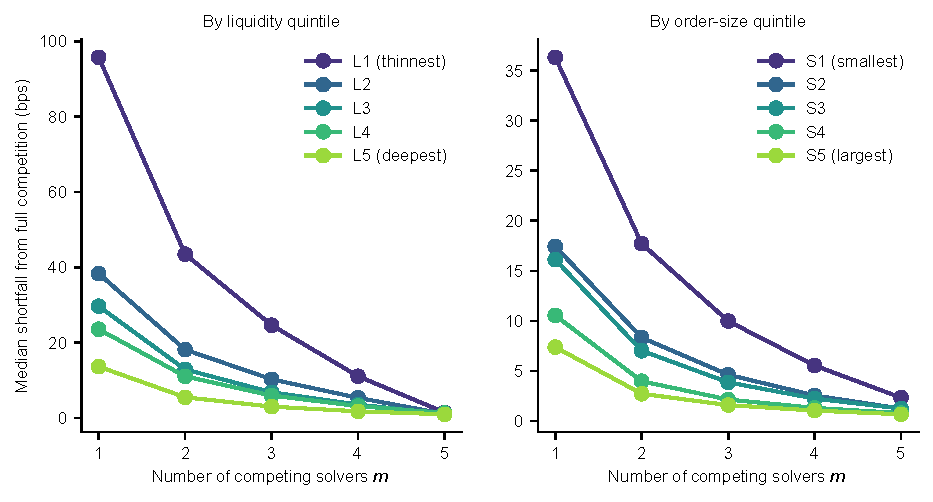
\includegraphics[width=0.92\linewidth]{figures/fig_liquidity.pdf}
\caption{The marginal solver curve along its two axes. Median competition shortfall $S(m)$, computed exactly per order (Eq.~\eqref{eq:subset}), by liquidity quintile of the counter-asset (left, L1 thinnest to L5 deepest) and by order-size quintile (right, S1 smallest to S5 largest); balanced panel of orders with $n \ge 5$ bidders, top 1\% of single-bidder shortfalls per group trimmed. Bids are held fixed throughout; the decline in $m$ is mechanical, while the magnitudes and the monotone ordering along both axes are the findings. The thinnest liquidity quintile contains 97 orders and is noisy in level.}
\label{fig:liquidity}
\end{figure}

\begin{table}[t]
\centering
{\fontsize{10}{12}\selectfont
\begin{tabular}{lrrrrr}
\toprule
Shortfall $S(m)$, bps (median) & $m=1$ & $m=2$ & $m=3$ & $m=4$ & $m=5$ \\
\midrule
Pooled          & 13.91 &  5.61 & 3.06 & 1.79 & 0.96 \\
L1 (thinnest)   & 95.74 & 43.45 & 24.61 & 11.06 & 1.45 \\
L2              & 38.31 & 18.12 & 10.25 & 5.33 & 1.08 \\
L3              & 29.65 & 12.87 & 6.78 & 3.53 & 1.05 \\
L4              & 23.54 & 11.03 & 5.94 & 3.15 & 1.29 \\
L5 (deepest)    & 13.62 &  5.47 & 2.99 & 1.75 & 0.96 \\
\midrule
Marginal value $\delta(m)$ & --- & 8.30 & 2.55 & 1.27 & 0.82 \\
\bottomrule
\end{tabular}}
\caption{The value of the marginal solver. Competition shortfall $S(m)$ relative to the order's full observed field, and its first difference $\delta(m)$, the basis points the $m$-th solver restores. All entries are medians. L1--L5 are asset quintiles of the liquidity metric of Section~\ref{sec:census}. Balanced panel, orders with $n \ge 5$ bidders; top 1\% of single-bidder shortfalls per quintile trimmed.}
\label{tab:shortfall}
\end{table}

Order size is the curve's second axis (Figure~\ref{fig:liquidity}, right panel): across order-size quintiles the median single-bidder shortfall falls monotonically from 36.3~bps for the smallest orders to 7.4 for the largest, and the gradient survives inside liquidity groups, from 20.8 to 8.0~bps within the deepest assets and from 75.1 to 23.9 within the second-thinnest. Small orders face material single-bidder exposure even where liquidity is deepest. The runner-up margin tells the same story in the cross-section, falling from 18.3~bps in the smallest size decile to about 1.1 in the largest while participation rises from 5.3 to 8.7 bidders.

\subsection{Niche leadership and the concentration of exposure}\label{sec:pivotal}
Who wins, and where, is the first test of the model's benchmark. Across the 479 counter-assets with at least a hundred settled orders, 21 of the 47 solvers are the modal best bidder in at least one, and the single busiest leader is modal in only 155 of them, a third; the typical asset's leader is best on 28 percent of its orders. Leadership is thus real, persistent, and \emph{niche-specific}, not the exchangeable draw a symmetric-entry model would produce~\citep{levin1994entry} and not one globally superior firm. This is the empirical footprint of positions (Section~\ref{sec:model-positions}): capacity that lives in an asset, held by whichever firm currently occupies it.

The same niches concentrate the fixed-bid exposure. Who provides this value on the recorded bids? For each order I attribute the runner-up margin to the solver making the best offer, weight by order notional, and aggregate (Section~\ref{sec:model-objects}). Over twelve months this aggregate fixed-bid exposure, the user loss if, order by order, the best bidder had been absent with all other bids unchanged, is about 2{,}586~ETH. Its distribution across solvers is stark (Figure~\ref{fig:pivotal}): the top solver carries 44.5 percent while being best on 53{,}615 orders at a median margin of 2.0~bps; the top two carry 62.4 percent, the top three 69.0. The Herfindahl of this exposure, 0.244, substantially exceeds the Herfindahl of best-offer volume, 0.147. The two indices measure different objects, who would be missed against who wins, and the comparison shows the first is far more skewed than the second, a dimension of market structure that share-based statistics, the only ones the prior literature could compute, do not capture. Whether this measured exposure translates into realized dependence is exactly the question Section~\ref{sec:exitstudy} puts to an experiment, and the answer there qualifies this subsection's reading. One mechanical caveat applies to all best-offer-based objects: under batch-level selection the winning execution sits below the order's best offer on 8.3 percent of orders, by 1.73~bps at the median, so the recorded best offer slightly overstates what the order realized; the realized-quality outcomes used in Sections~\ref{sec:exitstudy} and~\ref{sec:time} are measured on executions and unaffected.

\begin{figure}[t]
\centering
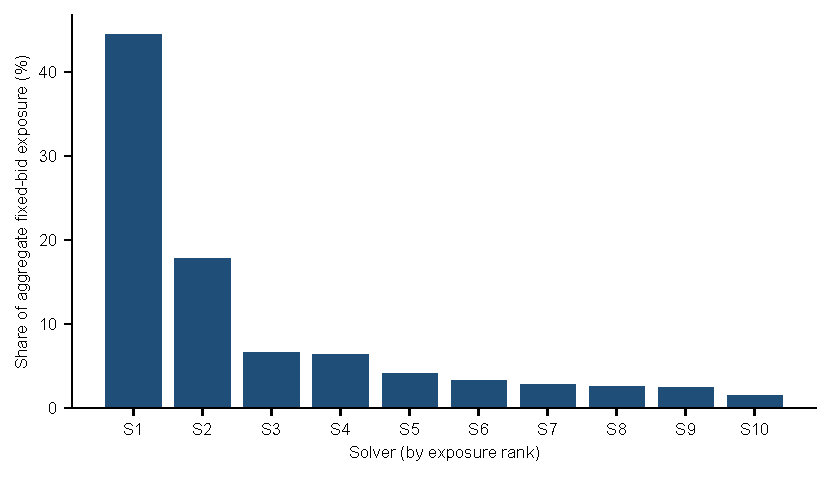
\includegraphics[width=0.88\linewidth]{figures/fig_pivotal.pdf}
\caption{Concentration of fixed-bid exposure. Each solver's share of the aggregate notional-weighted runner-up margin (the user loss its individual absence would impose, holding all other bids fixed), top ten solvers of 47. The top two solvers carry 62 percent of measured exposure; Section~\ref{sec:exitstudy} shows this exposure is contestable, not realized dependence.}
\label{fig:pivotal}
\end{figure}

\subsection{Does exposure bind? Substitution through the December churn}\label{sec:exitstudy}
Whether the fixed-bid measure captures realized dependence is a question the market itself answered when the field churned in December 2025; this subsection uses the churn to check the measure, and Section~\ref{sec:time} takes up the reform that plausibly caused it. The field's movements let the data speak without holding bids fixed (Figure~\ref{fig:cip74}). Across the thirteen sample months, the median bidder count and the median runner-up margin co-move with correlation $-0.73$. The sharpest movement is a December 2025 wave of three solver exits, arriving in the effective month of the CIP-74 reward reform and plausibly part of its repricing (Section~\ref{sec:time}): the median field thinned from six bidders in November to three at the February trough while the monthly median margin widened from 2.0 to 4.3~bps, and a wave of entries between February and April 2026, six solvers crossing the activity threshold, rebuilt the field to eight bidders by August and compressed the margin to 1.4~bps. The widening into the trough, about 2.3~bps, is close to what Table~\ref{tab:shortfall}'s within-order curve implies for thinning a five-bidder field to three, 2.1~bps. I read this as consistency between the fixed-bid measure and market dynamics, not as causal identification, because the aggregate series has no control group. The cross-section supplies one.

\begin{figure}[t]
\centering
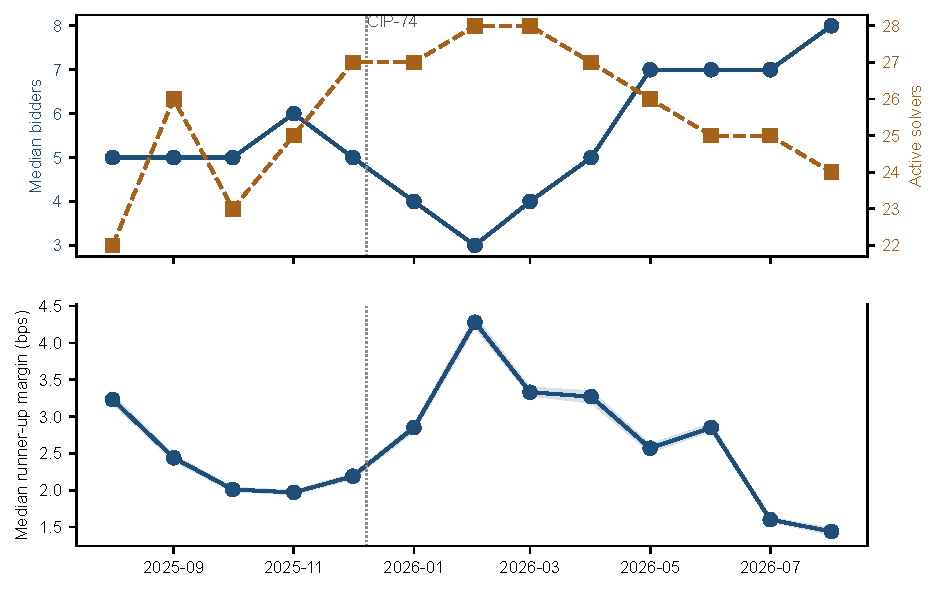
\includegraphics[width=0.95\linewidth]{figures/fig_cip74.pdf}
\caption{Competition and prices over time. Top: median bidders per order (solid, left axis) and active solvers per month (dashed, right axis). Bottom: monthly median runner-up margin. Dotted line: CIP-74 (8~December 2025). The December 2025 exit wave and the spring 2026 entry wave move participation and margins in opposite directions; the monthly correlation between median bidders and median margin is $-0.73$.}
\label{fig:cip74}
\end{figure}


If the fixed-bid exposure measure of Section~\ref{sec:pivotal} captured realized dependence, the counter-assets where the exiting solvers had been most often best should have deteriorated most. I test this directly. The three exiters were, in the three pre-exit months, the best or second-best bidder on 16 percent of all orders; exposure varies sharply across counter-assets, from over 90 percent for the most exposed to essentially zero. I define treated assets as those with at least 25 percent pre-exit top-two exposure (48 assets, median exposure 42 percent) and controls as those below 5 percent (270 assets), on a counter-asset by month panel with equal asset weights. Outcomes are the mean bidder count, the median realized price improvement of executed orders against a routed AMM counterfactual pinned to each order's settlement block (winsorized at $\pm 100$~bps), and the median runner-up margin; the specification removes counter-asset and liquidity-stratum-by-month fixed effects, with strata recut as quintiles of the liquidity metric over the analysis assets so each stratum holds treated and control assets, and standard errors clustered by counter-asset.

The result is a precisely estimated absence of any differential effect, and it is informative. In the three impact months the treated assets lost \emph{no} bidders relative to controls ($-0.05$, standard error $0.18$), realized price improvement did not differentially fall ($-0.9$~bps, standard error $4.7$), and the runner-up margin did not differentially widen ($+1.9$~bps, standard error $2.6$); the event-time paths (Figure~\ref{fig:exitstudy}) are flat through the episode, with no pre-trend and no break. Losing solvers that had been top-two bidders on nearly half of a treated asset's orders left no detectable mark on that asset relative to others. Substitution absorbed the exits at the asset level, and directly so: of the 32 niches the departing solvers had led before the exit, 25 were reoccupied by a solver \emph{new} to that niche, with a median lag of zero months, the vacancy filled within the first post-exit month. The positions outlived their occupants. Meanwhile the aggregate field thinned and aggregate margins widened, and no asset class escaped it, which is exactly what the cross-section implies when the treatment is near-universal in intensity and individual suppliers are replaceable.

This is the signature of Proposition~\ref{prop:occupancy}. Leadership was persistent and niche-specific (Section~\ref{sec:pivotal}), so under firm-attached asymmetry~\citep{maskin2000asymmetric} the exit of a niche's leader should have removed its strong distribution and hurt exactly there; instead the niche was reoccupied and its outcomes held, because the capacity belonged to the position, not the firm. Two conclusions follow. First, the fixed-bid exposure measure of Section~\ref{sec:pivotal} is an \emph{upper bound} on realized dependence: it prices what would be lost if bids stood still, and reoccupation shows they do not. Second, what binds is not the identity of any solver but the aggregate depth of the field, which did fall market-wide for a quarter until firm formation restored it, the slow margin of Remark~\ref{rem:twospeeds}. Competition matters; competitors are replaceable.

\begin{figure}[t]
\centering
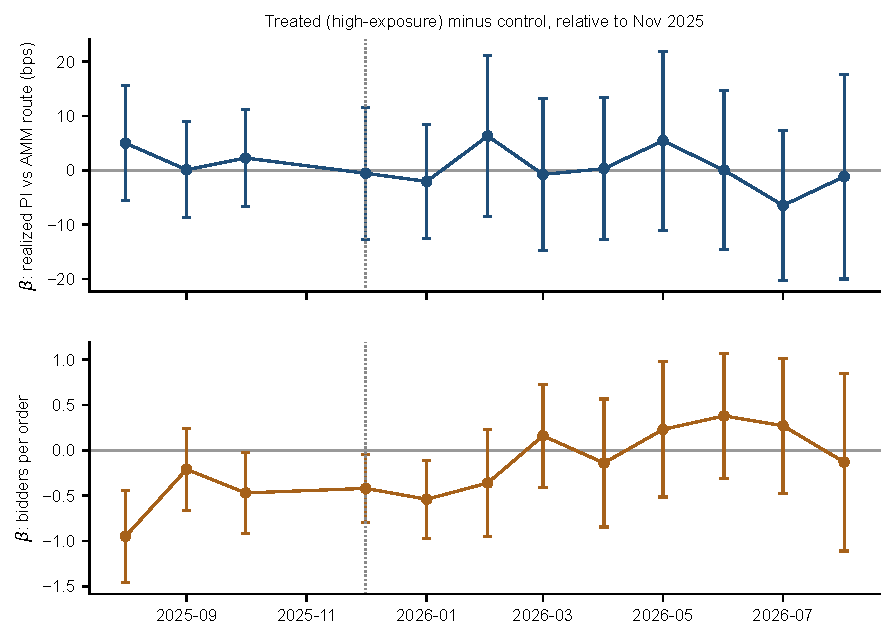
\includegraphics[width=0.92\linewidth]{figures/fig_exitstudy.pdf}
\caption{The exit experiment. Event-time differences between treated (high-exposure) and control counter-assets, relative to November 2025, with 95 percent confidence bands: realized price improvement against the routed AMM counterfactual (top) and bidders per order (bottom). Counter-asset and liquidity-stratum-by-month fixed effects; standard errors clustered by counter-asset. Assets most exposed to the December exiters show no differential deterioration in either outcome.}
\label{fig:exitstudy}
\end{figure}

\subsection{The natural experiment: CIP-74 and the participation channel}\label{sec:time}
CIP-74 is the paper's natural experiment: a governance-dated, real-world repricing of solver rewards, set against the participation-channel prediction of Proposition~\ref{prop:neutrality}. The membership churn just documented is timing-consistent with that channel doing the responding: the three exits and three entries of December land in the reform's effective month, and the entry wave that rebuilt the field follows within a quarter. I read the exits as plausibly a response to the repriced rewards, though motives are unobservable in these data. The proposition's two halves then both check out at the level where identification exists. Participation moved, active solvers rising from 23.6 to 26.2 per month and the single-bid share falling from 24.5 to 22.3 percent; and the predicted transmission to quality is small, the net participation change of about a quarter-bidder per order times the curve's $\delta$ near $n=6$ giving well under one basis point, comfortably inside the seven-basis-point bound that \citet{zhang2026incentives} estimates independently. His study reads the same reform through value capture and concentration; this one reads it through participation and margins, and the two are complements on one event.

The conditional-invariance corollary of Remark~\ref{rem:invariance} admits no direct test, for reasons the discussion summarizes; the mechanism itself supplies the test that works, and specifies it in advance. The pre-reform cap was fixed at 0.012~ETH per auction, truthfulness weakens exactly where the cap binds, and CIP-74 replaced it with a revenue-tied cap, so any bid-shading response to the reform should concentrate in assets whose auctions ran into the old cap. In the pre-reform months, 4.5 percent of orders sat in cap-binding auctions, single-winner auctions whose winner--runner-up solution score exceeded the cap. Classifying counter-assets by their pre-reform share of such orders and running the same asset-by-month design as Section~\ref{sec:exitstudy} (109 exposed assets against 121 zero-exposure controls), bidding margins show no differential response: $+1.7$~bps (standard error 4.5) in the transition and $+5.5$ (6.1) thereafter, and $+0.6$ under either halving or doubling of the cap threshold. Participation instead rose differentially in the previously cap-bound assets, $+0.8$ bidders per order (standard error 0.2), which is where the revenue-tied cap raises maximum rewards, the participation channel operating cross-sectionally, though an imperfect pre-trend keeps this reading suggestive. Realized price improvement in exposed assets declines after the reform, but exposure is classified from the same window as the pre-period outcome, so level reversion contaminates that coefficient and I do not interpret it. On its specified object the test is clean: no detectable bidding-margin response to the repricing, consistent with Proposition~\ref{prop:neutrality} and with truthful bidding surviving the reform.


% ===========================================================================
\section{Discussion}\label{sec:discussion}
% ===========================================================================

\paragraph{A market contestable in positions, slow in depth} The results obey one law, and the extension of Section~\ref{sec:model-positions} explains it: in this market adjustment runs through participation, because competition attaches to positions and firms are their transient occupants. Two firms carry 62 percent of fixed-bid exposure and leadership is persistent in asset niches, the picture that share-based concentration reads as fragility; yet when the most-relied-upon solvers left, their niches were reoccupied and outcomes there held, exactly Proposition~\ref{prop:occupancy}. What the market cannot substitute away is aggregate depth: the median field thinned from six bidders to three for a quarter and margins roughly doubled until firm formation rebuilt it, the slow margin of Remark~\ref{rem:twospeeds}. Niches are contestable in the sense of \citet{demsetz1968utilities} and \citet{baumol1982contestable}; depth is a slow state variable, the slow-moving capital of \citet{grossman1988liquidity} and \citet{duffie2010capital} and the resilience \citet{atkeson2015entry} leaves exogenous. Competition matters; competitors are replaceable.

\paragraph{What this says to traditional markets} The reading exports, because the two poles it rejects are the standard ones and the general fact behind the extension, execution technology specialized by instrument, is not on-chain-specific. In classic dealer markets losing a provider did hurt: dealer exits permanently widened spreads~\citep{wahal1997entry}, and removing a designated market maker degraded liquidity where removing a voluntary one did not~\citep{clarkjoseph2017designated,venkataraman2007value}. The extension says why the sign flips here, positions carried obligations, thin entry margins, or correlated stress in those settings and were not contestable, whereas an informal solver niche is; so the paper's verdict is the first contestability test of a market-making structure, a hypothesis outside banking~\citep{baumol1982contestable} that had gone untested, and it yields a portable prediction: where provider positions are contestable, share-based concentration overstates fragility and the depth of the field is the statistic to watch. The measured curve is, along the way, Stigler's value-of-search schedule~\citep{stigler1961information} drawn at every $m$ from observed quotations rather than an assumed distribution, and it gives the extra-bidder principle of \citet{bulow1996auctions} field magnitudes; it also reconciles the dealer-count evidence, tight count--margin co-movement here against collusive spreads among thirty visible NASDAQ dealers~\citep{christie1994nasdaq}, as the count measuring competition only jointly with the mechanism.

\paragraph{How much competition is enough, and who should watch} Three to five independent bids capture nearly all of competition's value; beyond five the marginal bidder is worth under a basis point for the typical order. Because the bid record is public and the computation deterministic, any user, venue, or supervisor can locate an order on the curve. Where best execution is a duty owed by an intermediary~\citep{mifid2,finsa,finra5310}, competition is its only substitute in a broker-free market, and the statistic to audit is the depth of the field, informative and publicly recomputable though not a proven sufficient statistic, since its content rests on the mechanism keeping bids competitive. This gives the argument that verifiable execution can stand in for conduct regulation~\citep{le2026fairness} a concrete object: verify not the winning price but the depth of the field behind it. For entrants the runner-up margins are the invitation, pricing the rent a firm with genuine capacity could earn precisely where niches are thin, and the substitution result is the entrant's reassurance and the incumbent's warning at once. I leave the business-model economics to future work; the map of where competition is scarce is drawn here.

% ===========================================================================
\section{Limitations}\label{sec:limits}
% ===========================================================================

Six limitations bound the claims. First, positions are operationalized at the counter-asset level, a coarse shadow of the true technology bundle, since a solver's edge may span correlated assets or a shared integration; the leadership and reoccupation evidence should be read as the asset-level footprint of positions, not a direct measurement of them. Second, the fixed-bid counterfactuals rest on a maintained idealization. Bids-as-capacities is motivated by the runner-up-keyed reward, but the production mechanism's caps and batch selection blunt the argument, and the exit experiment shows directly that participation adjusts; the cap-exposure test finds no bidding-margin response to the reform, which supports the idealization but is a bounded null, not proof, so the thinning curve should be read as an exact statement about the recorded field and an upper bound on equilibrium dependence. Third, a per-order proposal inside a batch solution need not be independently feasible once other orders change, so batch coupling qualifies not only bidding incentives but the feasibility of the counterfactual assignments themselves. Fourth, participation is endogenous: solvers choose which orders to bid on, so cross-sectional comparisons of $n$ conflate order attractiveness with competition, which is why the headline objects are within-order computations and the identified result is a designed contrast rather than a regression on $n$. Fifth, the census covers one venue, one chain, one quote asset, and only settled orders; the fill-rate series uses an expiry-based date proxy, and selection into settlement is not modeled. This is not incidental, since no other venue publishes losing bids, but it means external validity rests on the model, not the data: the curve's shape and the substitution finding are hypotheses for other markets, while the levels are this market's own. Sixth, solver identity is an on-chain address. If one operator runs several addresses, measured exposure concentration understates true concentration; the substitution result is robust in the reassuring direction, since consolidation would make the absorbed exits larger, not smaller, but the exposure rankings themselves carry the caveat.

% ===========================================================================
\section{Conclusion}
% ===========================================================================

What is one more competitor for a customer order worth? For fifty years the question could only be answered by inference, because the bids that lose are unobserved in every market that debated it. The first production market I know of to publish them permits a fixed-bid answer computed from the record, and then two experiments that discipline it. On the recorded bids, the answer is a great deal, quickly exhausted, and unevenly supplied: a single retained bidder would cost the median order 14 basis points, a second restores most of it, five make competition essentially complete, and the value is largest exactly where liquidity is thinnest. Measured exposure is concentrated in two firms. Yet when three major solvers left in December 2025, the assets most exposed to them fared no worse than any others, while the monthly median margin roughly doubled for a quarter as the field thinned and then recovered through entry; and when a reform repriced rewards, membership churned and participation moved while bids did not. Both experiments obey one law: adjustment runs through the participation margin. That law is what the paper's extension of costly-entry auction theory predicts once capacity attaches to positions rather than firms, making niches contestable while aggregate depth adjusts slowly. The fixed-bid measure is an upper bound; realized dependence attaches to the depth of the field, not to its members. Competition matters, competitors are replaceable, and in markets that have replaced the broker's duty with an auction, the depth of the field, publicly recomputable order by order, is where investor protection now lives.

% ===========================================================================
\section*{Acknowledgement}
% ===========================================================================

This research received no external funding.

% ===========================================================================
\section*{Author Contributions}
% ===========================================================================

N.B.\ is the sole author and performed all aspects of the study: conception, data collection, analysis, and writing.

% ===========================================================================
\section*{Conflict of Interest}
% ===========================================================================

The author declares no conflict of interest.

\bibliographystyle{unsrtnat}
\bibliography{references}

\end{document}
